% -- Implementation ---------------------------------------
\section{Implementation}
This section will cover some difficulties that came along during the lab. Section \ref{sec:debugging} will discuss our method for debugging and testing the working manner of the $\rho$-VEX, we will discuss some limitations we came accross in Section \ref{sec:fix} and \ref{sec:variable}. Important features to be considered were the difference in Endianess as will be discussed in Section \ref{sec:endian} and the reliability of the code, discussed in Section \ref{sec:reliable}.\\

The approach was to first let the \mcode{pixel.c} write mock up pixel data to the data memory. The instruction memory would already contain the bytecode of our extracted kernel as it was put in manually. The kernel would only contain a single public declared variable \mcode{pixel datamem[128];}. This array of pixels points towards the first address of the data memory as no other variables are declared and thus there are no competing variables after this data memory location. The pixel.map file and the hexdump proved this to be correct. By declaring a pointer to this data memory location we could determine the result on the $\rho$-VEX and write the result into this array at a set location where the \mcode{pixel.c} can read and return it. 

\subsection{Mock up pixels}
\label{sec:debugging}
In order to get some insight in how to communicate with the $\rho$-VEX we made \mcode{hexdumps} of the data memory and created a mock up version of the satd function using 2 pixels we took from the original application. In order to check where the $\rho$-VEX is writing the data, a debugging file \mcode{Debugging\_pixel.c} is created. When using this debugging file, \mcode{bytecode} is manually put into the instruction memory using \mcode{scp}, \mcode{ftp} and \mcode{put}. The data that is being sent from the MicroBlaze are two pre-defined pixels. By knowing the expected result and the possibility to write easy recognizable hexadecimal numbers such as \mcode{0xdead}, we can use the \mcode{hexdump} to examine the registers. The  hexdump in figure \ref{fig:testhex} portrays all but the first two bytes or our mock up bytes. These first bytes display the correct result written to a convenient addres \mcode{0x00}.

\subsection{Issues with the fix}
\label{sec:fix}
Halfway the lab, a fix was introduced. The physical address was supposed to be set to 0x120 and did not have to be passed on using \mcode{\_\_DATA\_START}. In order to make the $\rho$-VEX read the pixels in the data memory correct a pointer to the first logical address 0 would be enough. However as we would later discover this was not the case. The fix we applied did not adjust our working directory as it was designed to alter the tools folder in the home directory and we were working in a seperate folder. When we did find out, we changed the script of the fix to match our own tools folder, but it did cause some days delay. 

% --- Screenshot testpixels ---------------------------------
%\begin{figure}
%\centering
%	\begin{subfigure} [h] {0.5\textwidth}
%		\centering
%		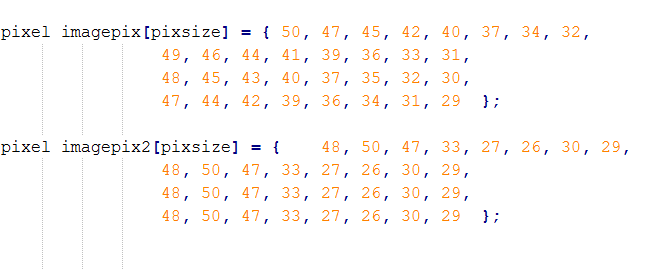
\includegraphics[width=300px]{Pictures/testpixels}
%		\caption{Test pixels defined in \mcode{pixel.c}}
%		\label{fig:test}
%	\end{subfigure}
%\quad
%\begin{subfigure} [h] {0.5\textwidth}
%	\centering
%	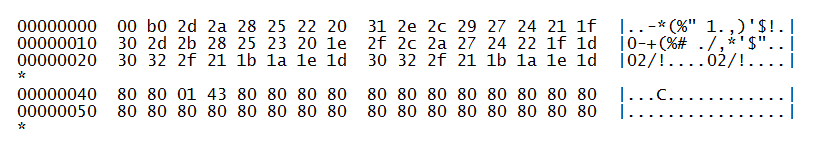
\includegraphics[width=300px]{Pictures/hextest}
%	%\caption{Hexdump of the testpixels (first two bytes incorrect)}
%	\label{fig:testhex}
%\end{subfigure}
%\quad
%\caption{Debugging the rovex with 2 }%
%\label{}%
%\end{figure}
%
% --- hexdump ----------------------------------
\begin{figure}[h] %
\centering
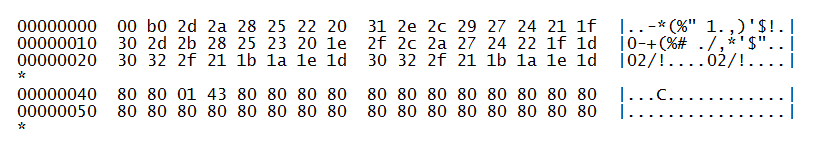
\includegraphics[height=80px]{Pictures/hextest}%
\caption{Hexdump of the kernel run with two mock up pixels}%
\label{fig:testhex}%
\end{figure}
%\subsection{Order of Variable Initialization}
%\label{sec:variable}
%After moving our code to the original x264 code and creating test pixels to be used for SATD calculation, a dump of the $\rho$-VEX data memory can been seen in figure \ref{fig:testhex}. As you can see, the first two byte are not matching. At first, we thought this could be because of the fact that another group was running their application at the same FPGA concurrently. However, the value of these bytes remained the same during several runs. 
%
%This unwanted write was caused by the initialization of the \mcode{sum} variable, that has type \mcode{short int} and was stored in the data memory before the pixel. When \mcode{pixel_satd_8x4} tried to find the pixels, it found \mcode{sum} instead of the pixels, causing the program to get stuck in a loop. When changes \mcode{sum} to not being initiazlied, \mcode{datamem} containing the pixels had the first spot at address 120.

\subsection{Endianness}
\label{sec:endian}
The MicroBlaze and the $\rho$-VEX understand basic operations like \mcode{open()}, \mcode{close()}, \mcode{read()} and \mcode{write()}. However, they differ in Endiannes. $\rho$-VEX operates in Little Endian, meaning the bytes are read from right to left, as seen in figure \ref{fig:little}. MicroBlaze, on the other hand, operates in Big Endian and thus reads the bytes from left to right (see figure \ref{fig:big} ). This becomes an issue when reading the \mcode{result} variable from the data memory, as we will get the bytes in reversed order. This problem is solved by manually reversing the order of the \mcode{result} bytes, realized by the piece of code in figure \ref{fig:swap}.

\begin{figure}[htb]
	\centering
	\begin{subfigure} [h] {0.5\textwidth}
		\centering
		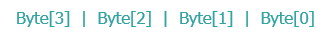
\includegraphics[width=150px]{Pictures/little}
		\caption{Little Endian}
		\label{fig:little}
	\end{subfigure}
	\quad
	\begin{subfigure} [h] {0.5\textwidth}
		\centering
		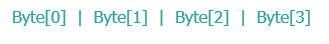
\includegraphics[width=150px]{Pictures/big}
		\caption{Big Endian}
		\label{fig:big}
	\end{subfigure}
	\quad
	\begin{subfigure} [h] {0.5\textwidth}
		\centering
		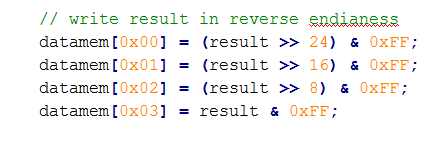
\includegraphics[width=150px]{Pictures/byteswap}
		\caption{Reversing the order of bytes}
		\label{fig:swap}
	\end{subfigure}
\caption{Different reading direction due to Endianness}%
\label{}%
\end{figure}

\subsection{Reliability of the code}
\label{sec:reliable}
When writing pixels to the data memory of the $\rho$-VEX, the data pointer is automatically increased. To ensure that \mcode{pixel.c} reads the correct result from the memory location we can use \mcode{lseek}, a system call that is used to change the location of the read/write pointer of a file descriptor. Using \mcode{lseek(data, 0, SEEK_SET)}, the pointer in the $\rho$-VEX moves to the address that is the start address from his point of view (thus, physical address 0x120). Translating the logical address 0 to the physical address 0x120 is done by the linker and is not of our concern. We also added some if statements that ensure that if memory locations are not opened correctly, they return \mcode{0xff} and print an error to the screen. These measures increase the reliability of the code. 
